% Document Styling
\documentclass[12pt]{article}
\usepackage[margin=1in]{geometry}
\usepackage{graphicx}
\graphicspath{{images/}}
\usepackage{booktabs}

\begin{document}

\title{EE 374N Homework 1}
\author{Ishan Shah}
\date{\today}
\maketitle

\section{Signal Processing}
\subsection{Understanding the Signals}
We can see that the raw signals are extremely noisy.

\begin{center}
    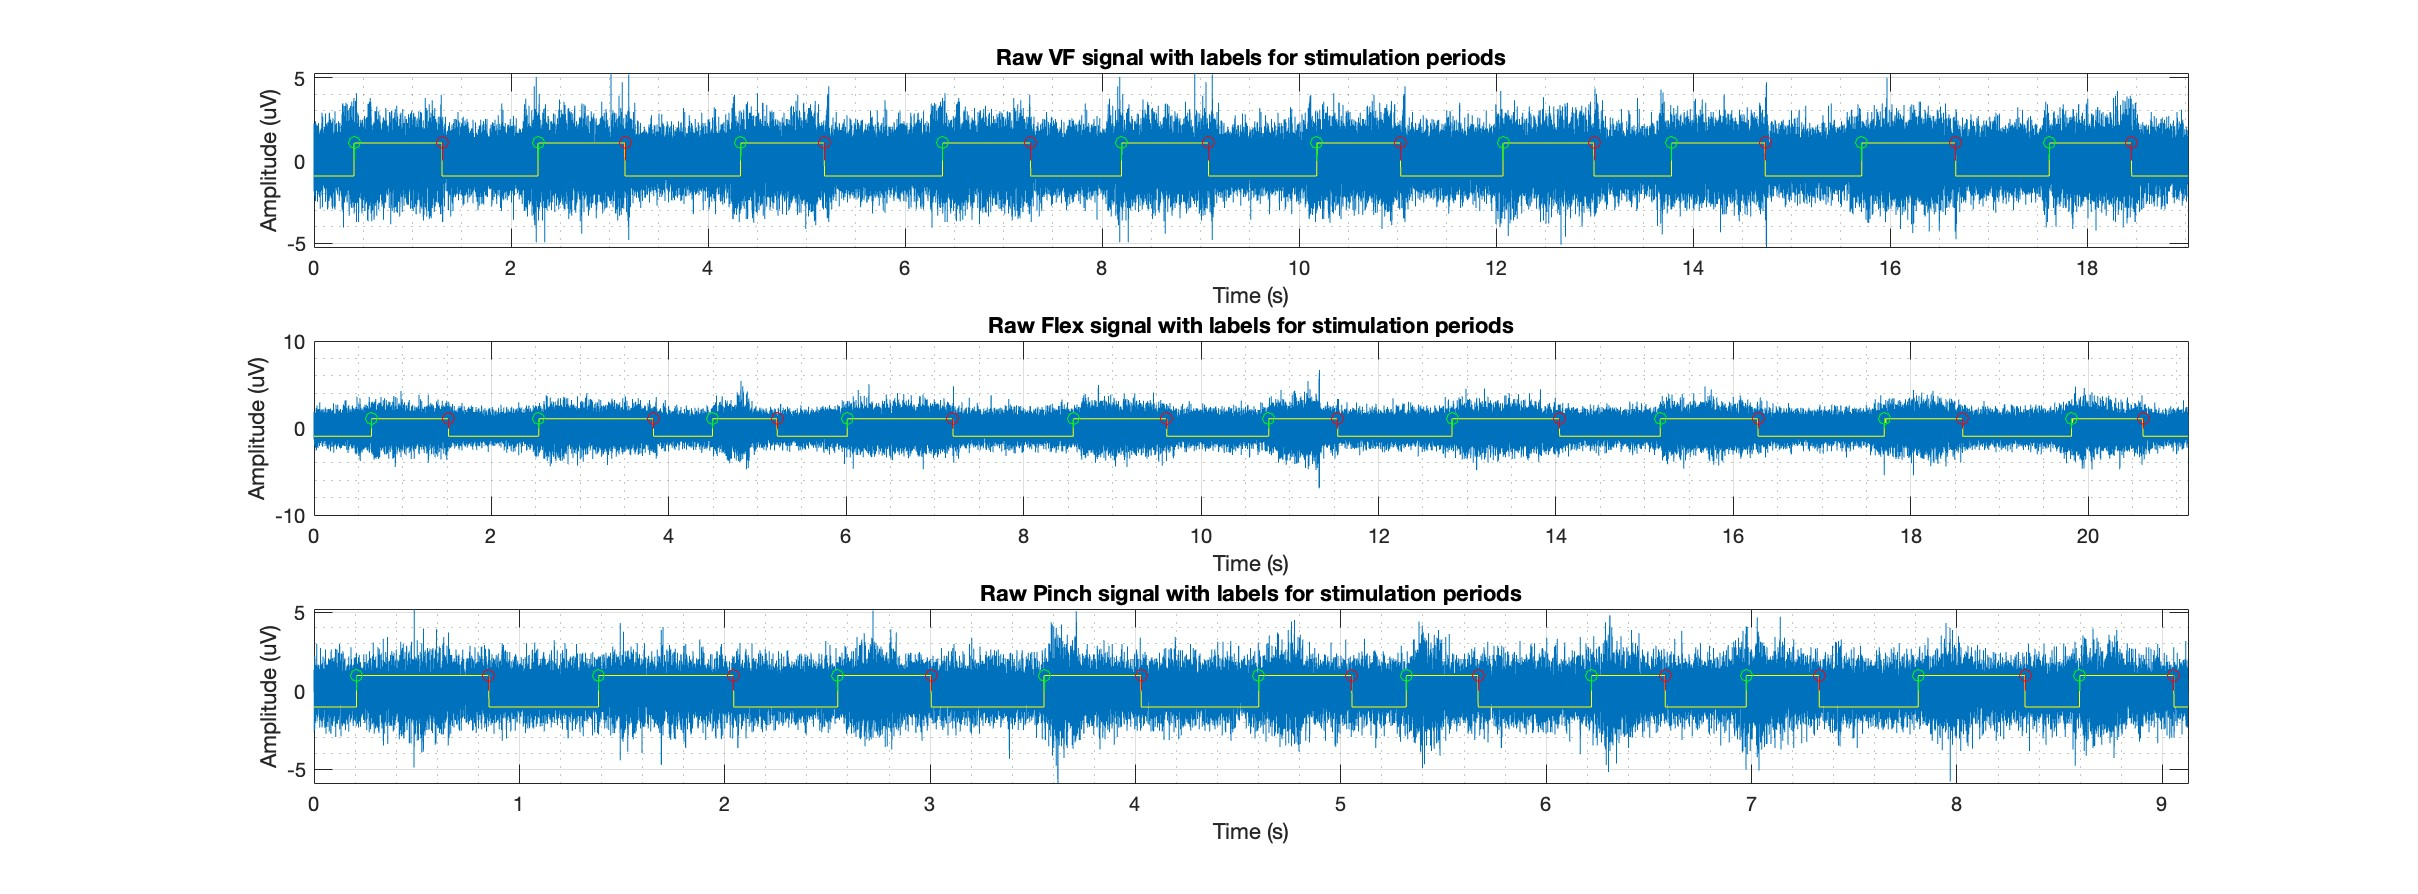
\includegraphics[width=\textwidth]{raw_signals.jpg}
\end{center}

The PSD estimate of the raw signals gives us a better understanding of the frequency content of the signals.

\begin{center}
    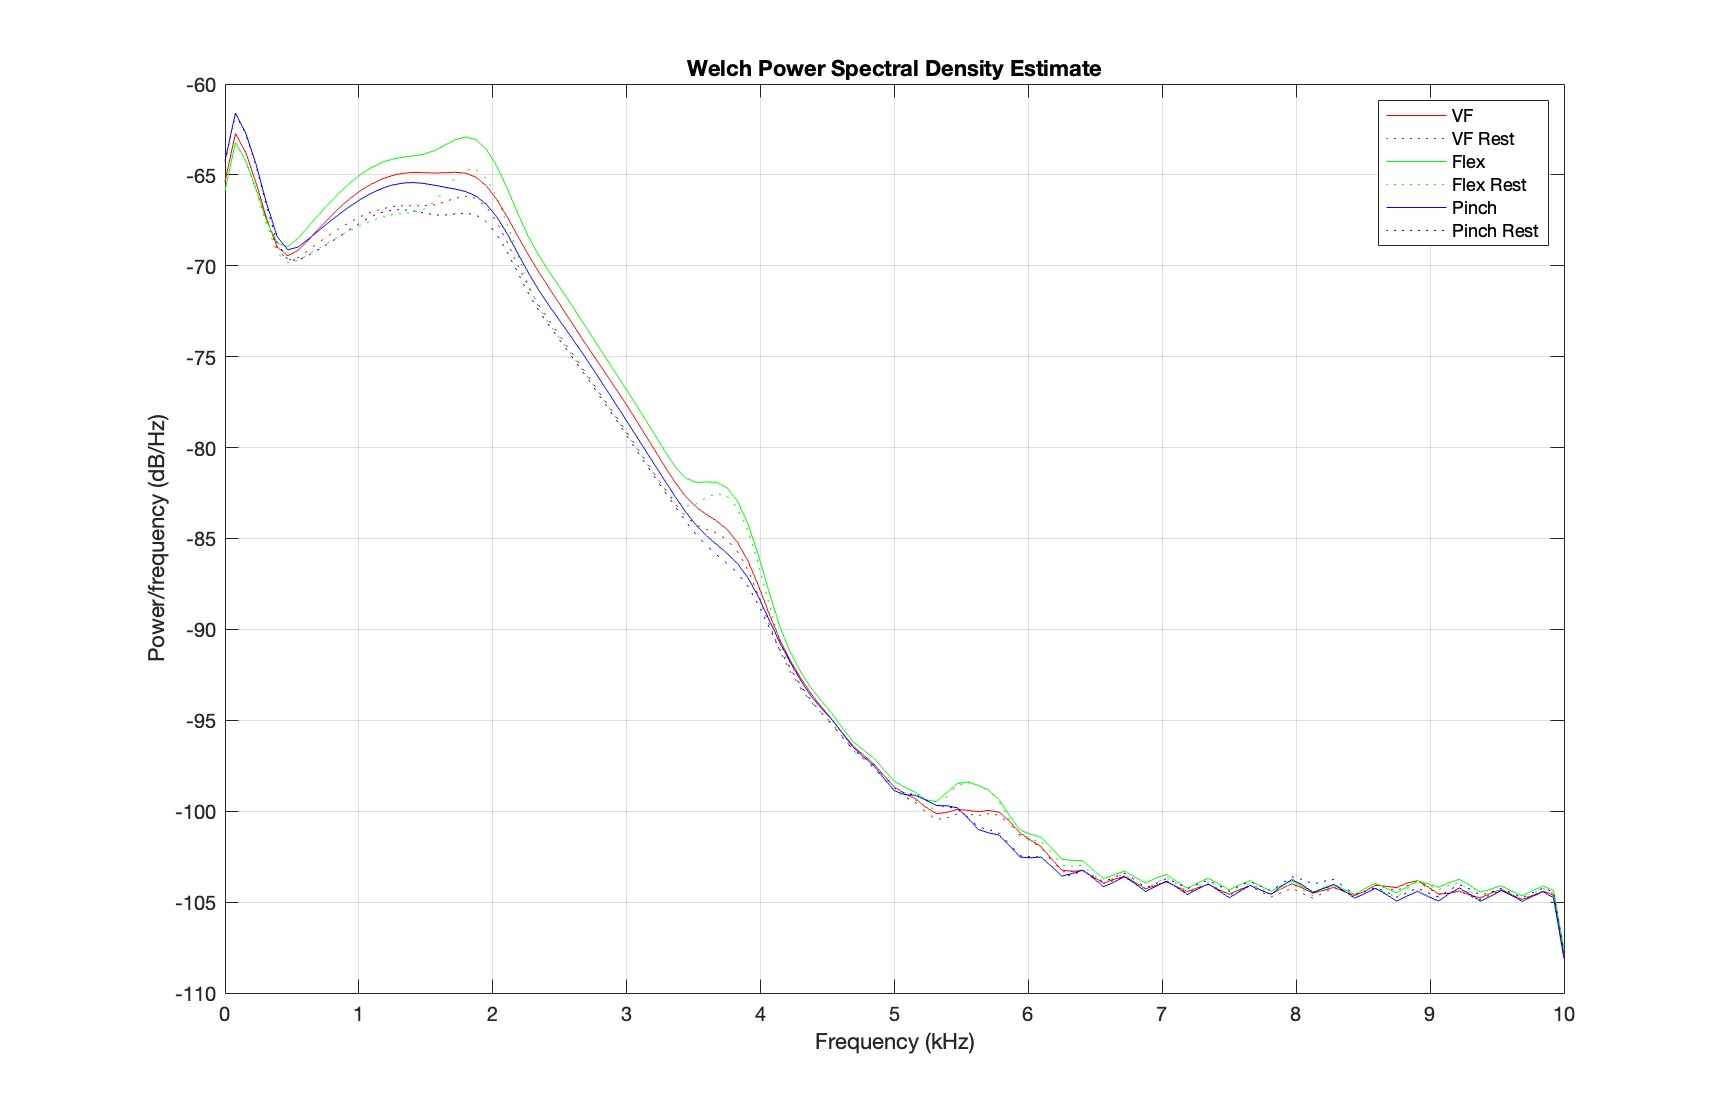
\includegraphics[width=\textwidth]{psd.jpg}
\end{center}

\subsection{Bandpass Filtering}
Based on the PSD graph, the most useful frequency range seems to be the 1 kHz to 2 kHz range. This range has mostly flat lines, which makes it easy to discriminate between the different signals. This is also the range with the maximum difference between each stimuli and their corresponding rest periods.

This range aligns decently well with the 0.8 kHz to 2.2 kHz range described in the paper. Filtering using this range is useful because it allows us to focus on the most relevant frequencies, which makes it easier to differentiate between the signals.

\begin{center}
    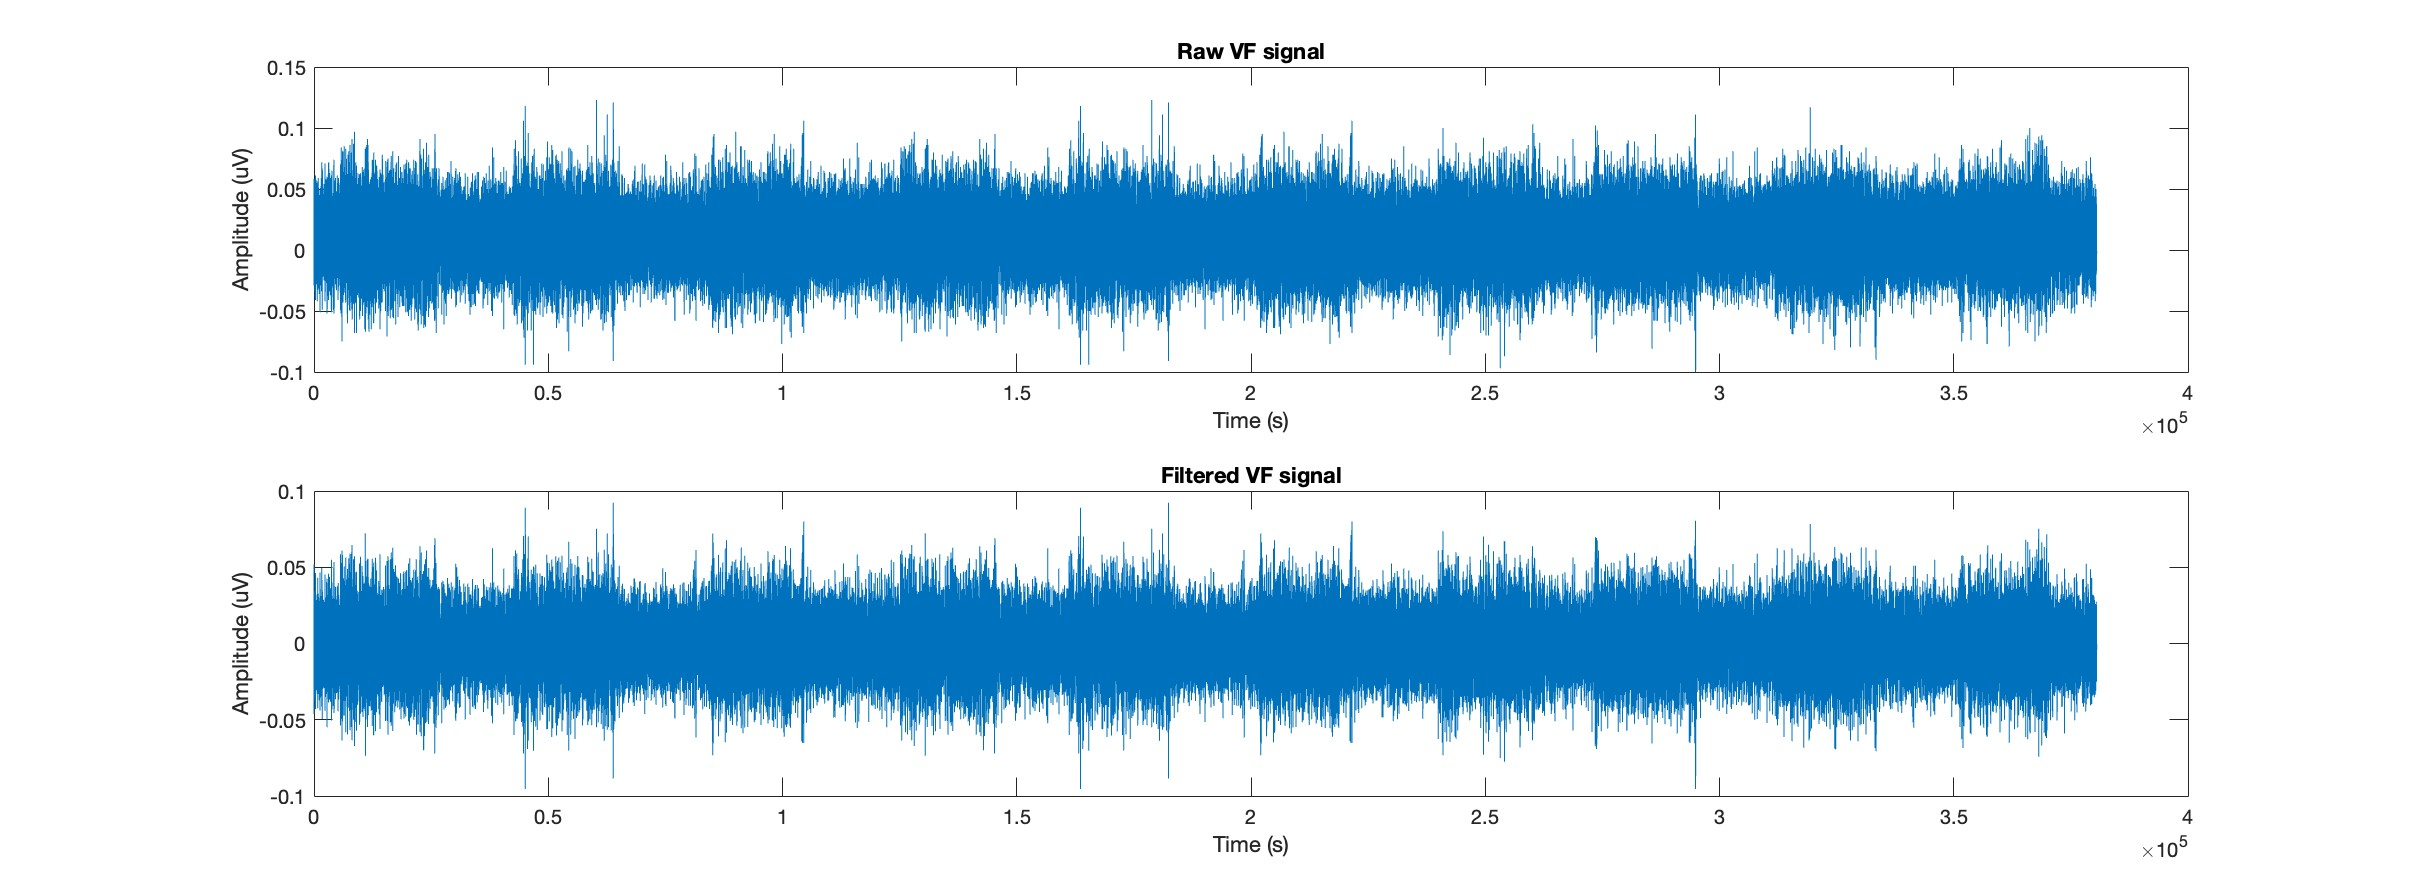
\includegraphics[width=\textwidth]{filtered_vf_signal.jpg}
\end{center}

The key difference we observe between the VF stimulation before and after filtering is that the filtered signal is much more consistent. The unfiltered signal has a lot of noise, which makes it difficult to distinguish between the different stimuli. The filtered signal has had its high-frequency components removed leaving the lower-frequency signals, which aligns with the 0.8 kHz to 2.2 kHz range we identified earlier in the PSD estimate.

\begin{center}
    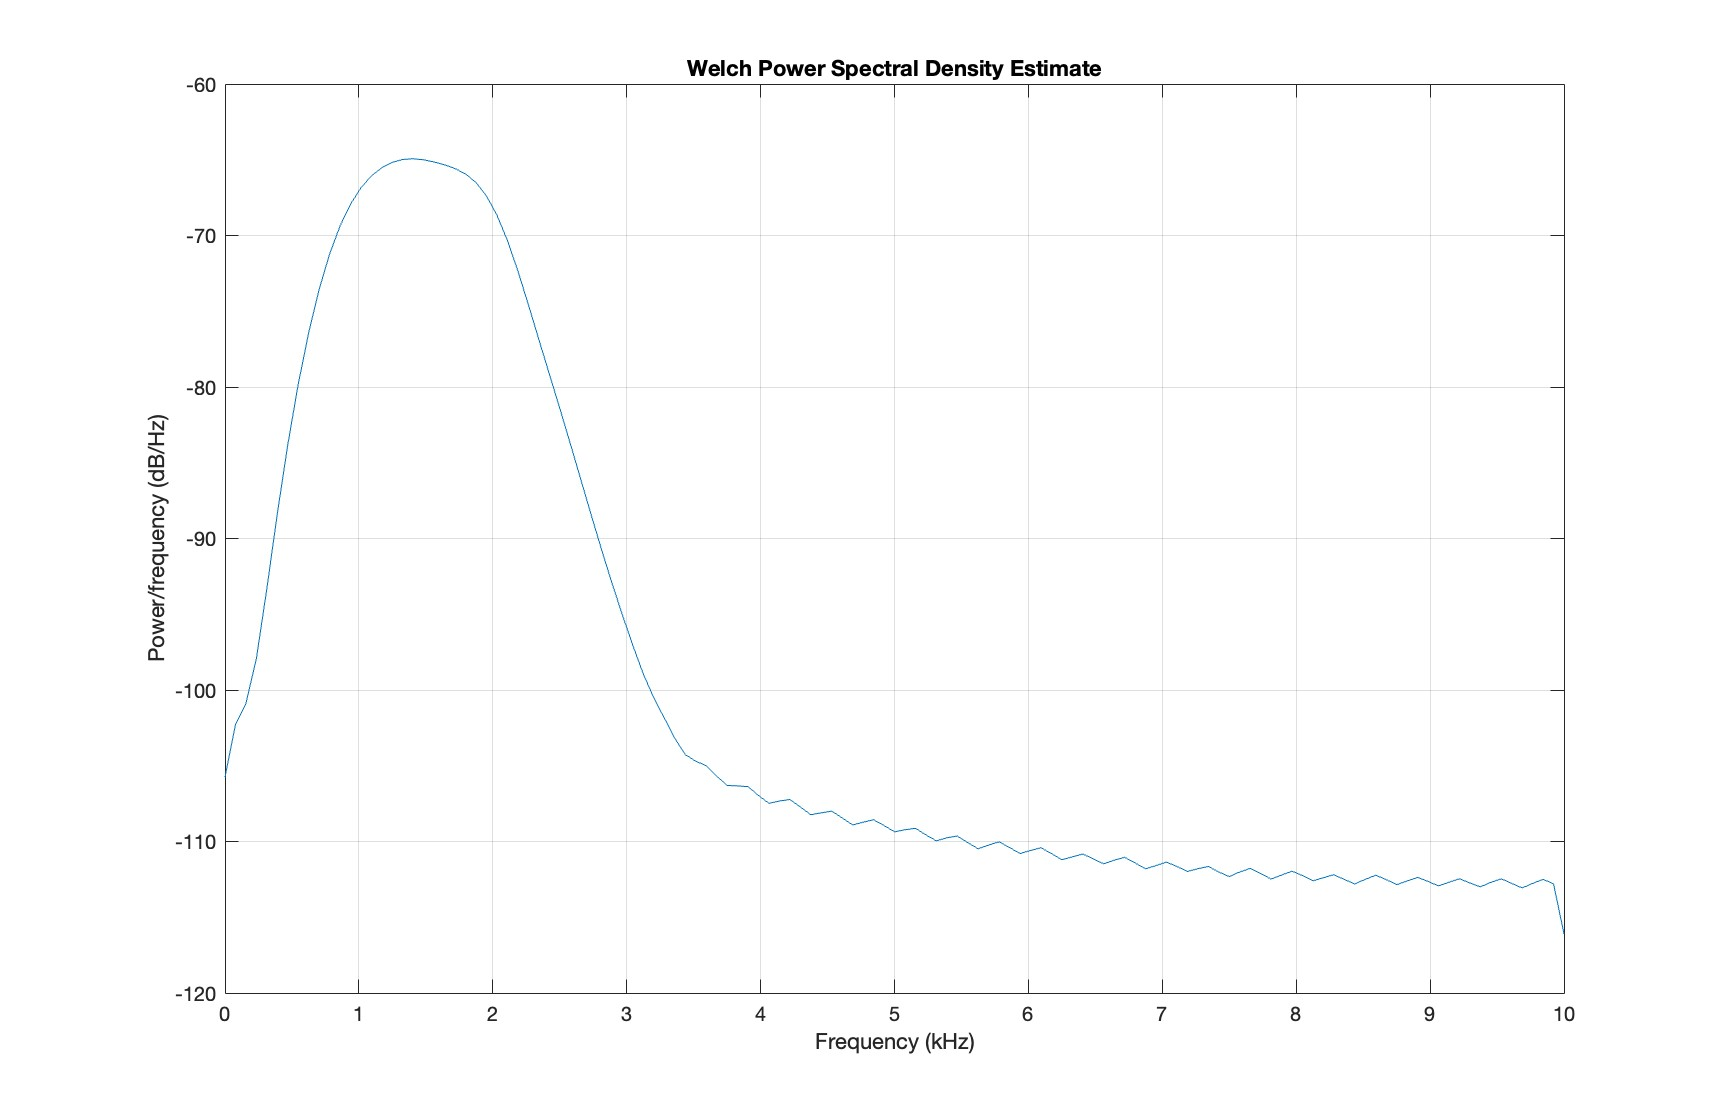
\includegraphics[width=\textwidth]{filtered_vf_psd.jpg}
\end{center}

The updated PSD estimate of the VF signal shows that we've mainly retained the signal in the 0.8 kHz to 2.2 kHz range.

\section{Feature Extraction}
\subsection{MAV and VAR Features}
On a cursory glance of the different VF plots, we can see that a window size of 0.1s and 0\% overlap gives us a signal that lines up decently well with the stimulation period. Generally, a smaller or larger window size than this gives us a signal that is either too dense or too sparse and a larger overlap creates a noisier signal. This choice of window size and overlap should also generalize to the other stimuli.

\begin{center}
    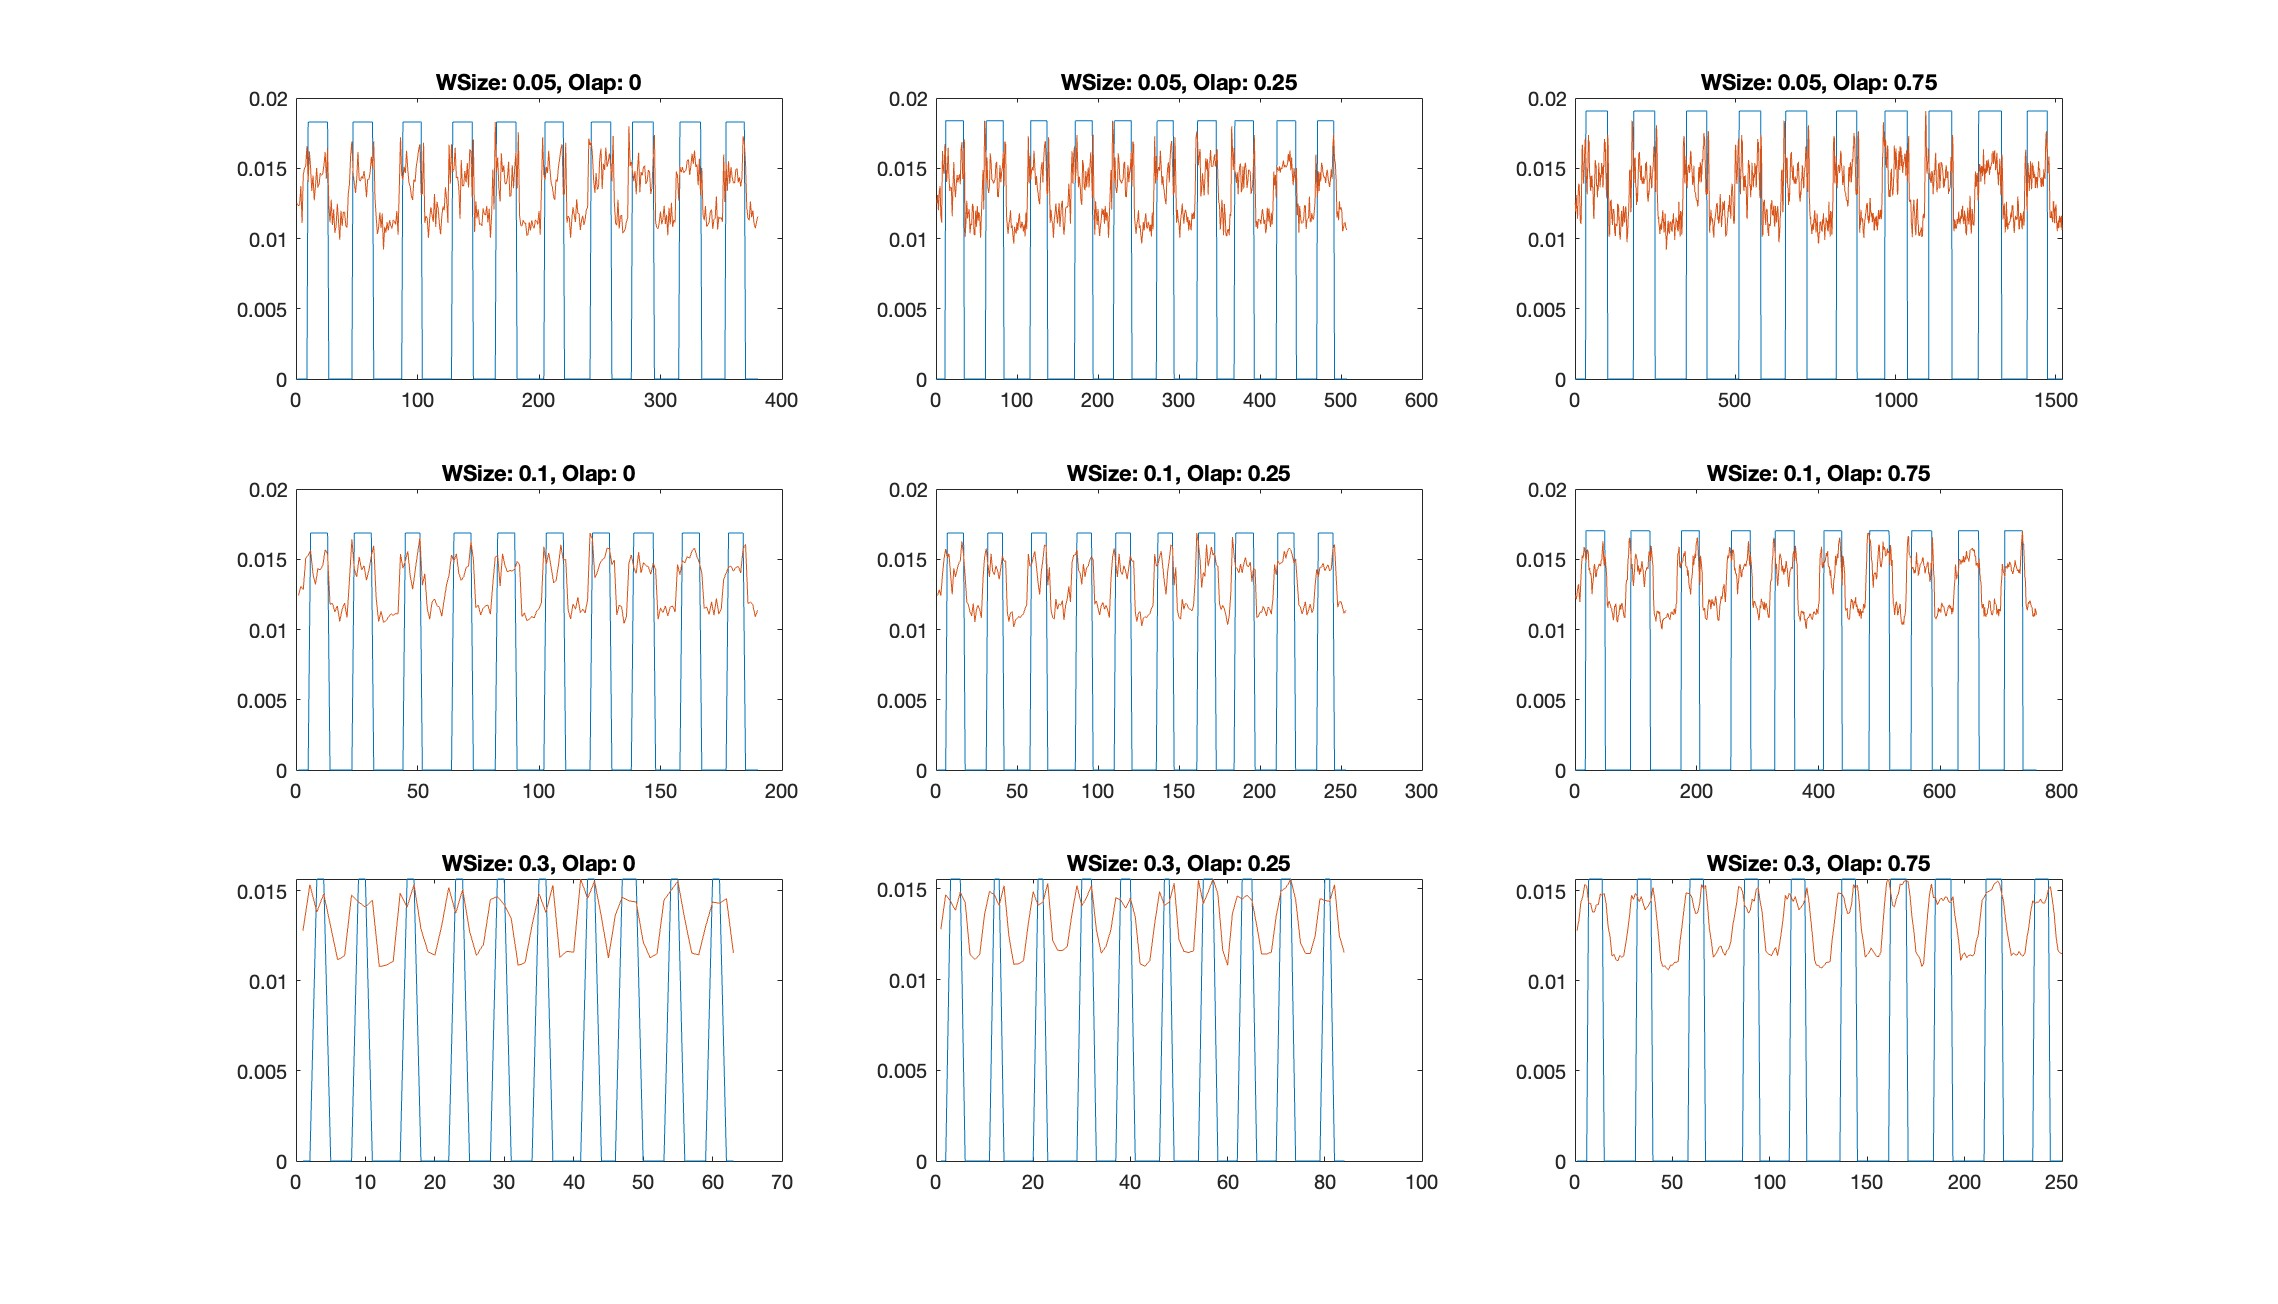
\includegraphics[width=\textwidth]{wsize_olaps_mav.jpg}
    VF MAV Features
\end{center}

\begin{center}
    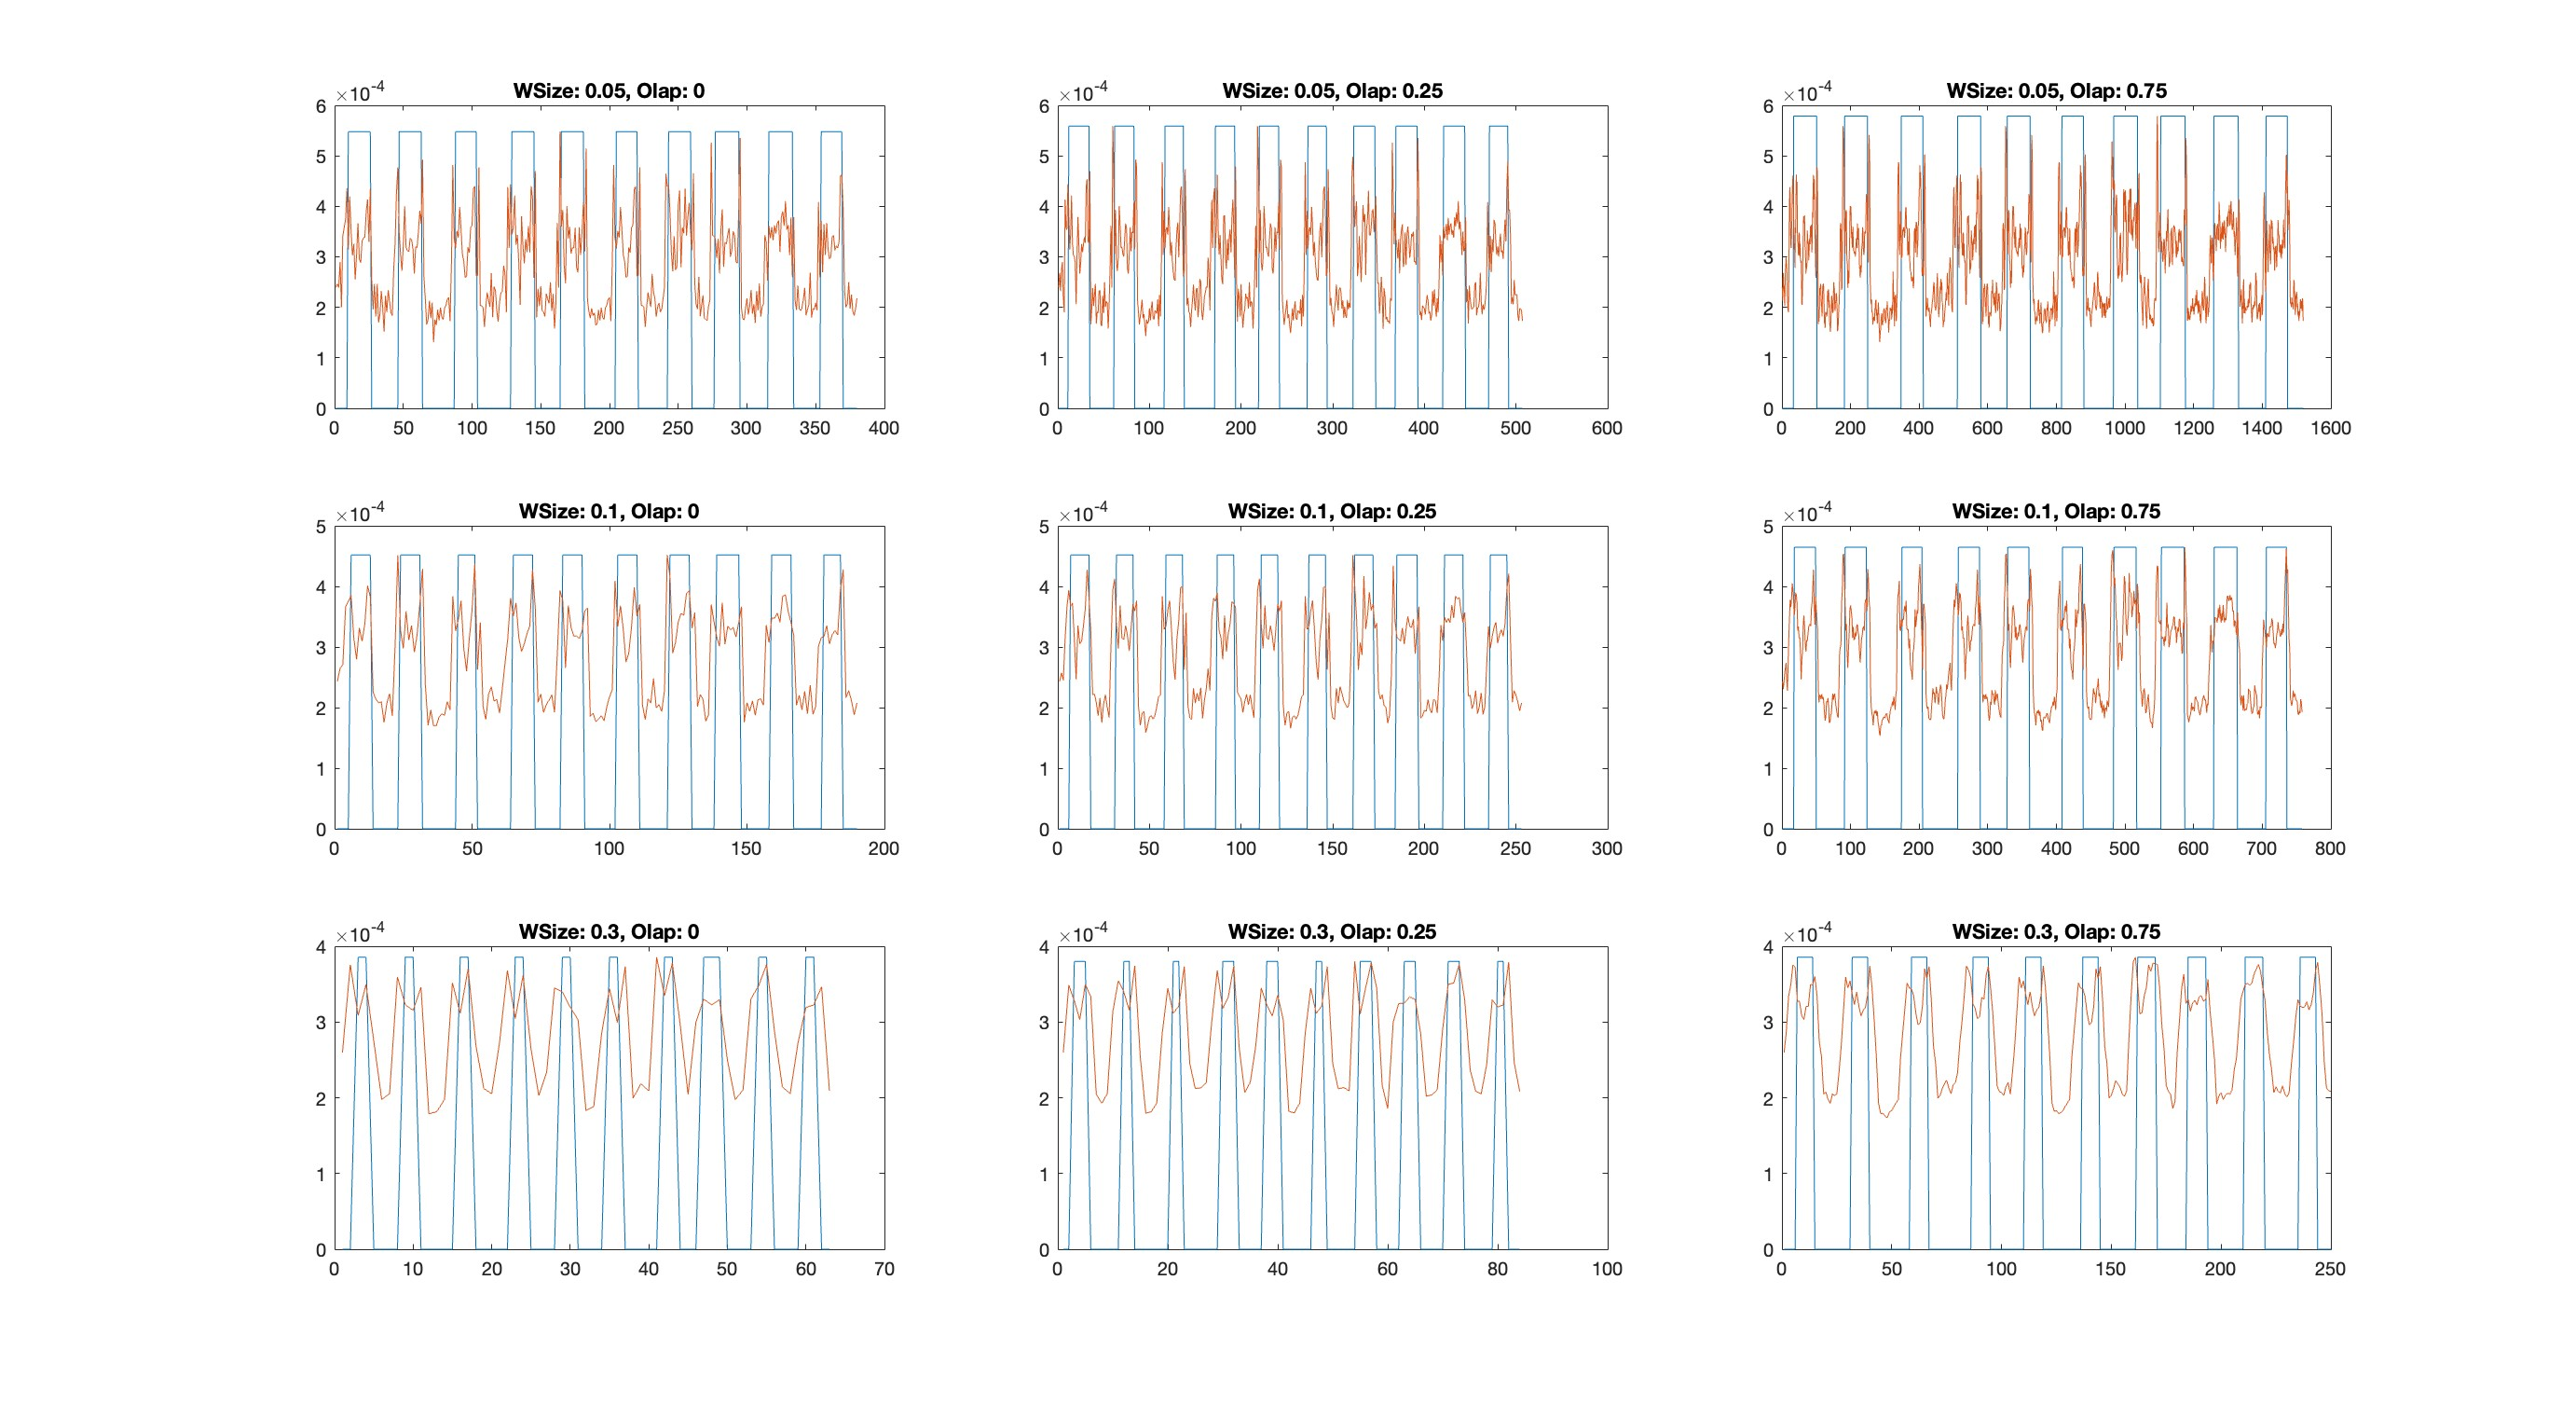
\includegraphics[width=\textwidth]{wsize_olaps_var.jpg}
    VF VAR Features
\end{center}

A better approach than mere visual inspection would be to use hyperparameter tuning by trying to optimize a function over the space of possible window sizes and overlaps. This function could be the absolute value difference between the signal and the stimulation period. We could then use the window size and overlap that gives us the minimum value of this function.

Additionally, we may want to consider how a larger window size would cause us to expend more time and compute. This means there is a tradeoff between computation efficiency and window size that is important to keep in mind. 

Now that we know the optimal window size and overlap, we can compare MAV and VAR for VF, Flex, and Pinch. The following graphs all use a window size of 100ms and 0\% overlap.

\begin{center}
    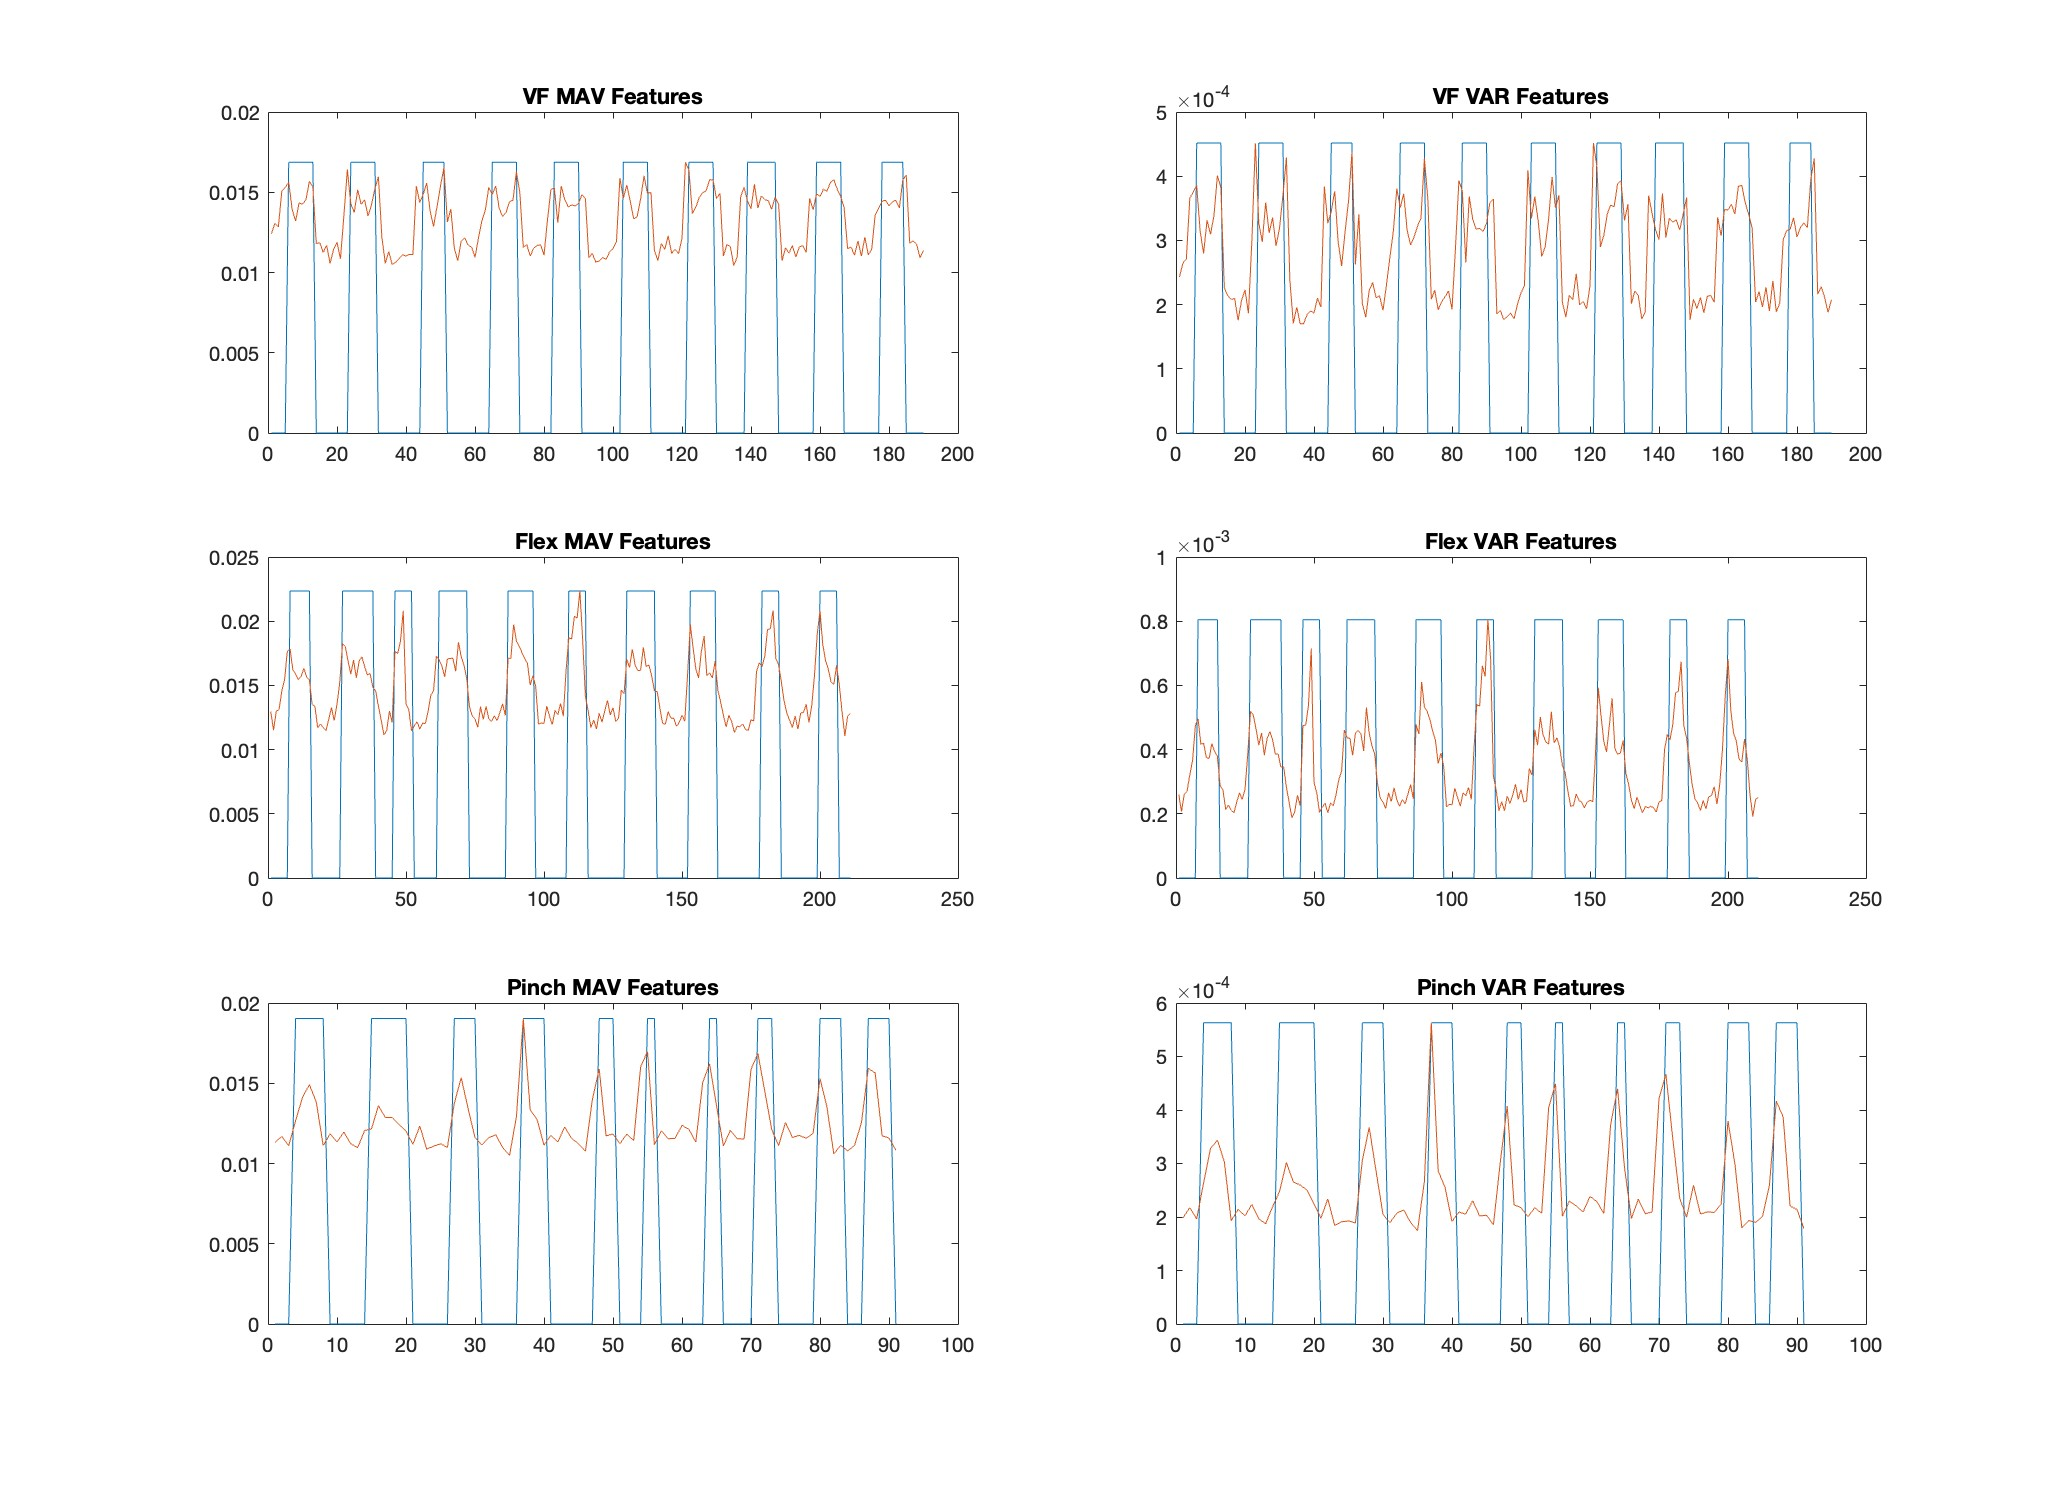
\includegraphics[width=\textwidth]{mav_var_comparison.jpg}
    MAV vs. VAR
\end{center}

It appears that VAR is a better feature than MAV for all three stimuli. This is because the VAR stimuli features are easier to distinguish from the rest periods than the MAV features.

\subsection{Feature Selection}
We can compute a signal-to-noise ratio (SNR) for each feature to determine which one is more useful.

\begin{center}
    \begin{tabular}{@{}lll@{}}
        \toprule
            & MAV    & VAR    \\ \midrule
        VF    & 1.4955 & 2.7377 \\
        Flex  & 2.3147 & 4.7261 \\
        Pinch & 1.1612 & 2.5630 \\ \bottomrule
    \end{tabular}
\end{center}

Based on this table, we can see that VAR is a better feature than MAV for all three stimuli since the SNR indicates that the feature is more informative. It also appears that the Flex signal is easiest to detect using a classifier since it has the highest SNR of all the classes. One physiological explanation of this from the Raspopovic paper is that SNR is proportional to the diameter of fibers conducting the corresponding stimuli. Therefore, proprioceptive signals from the Flex muscles are easier to detect than the other stimuli.

\section{Classification}
The confusion matrices for the different classifiers are shown below.

\begin{center}
    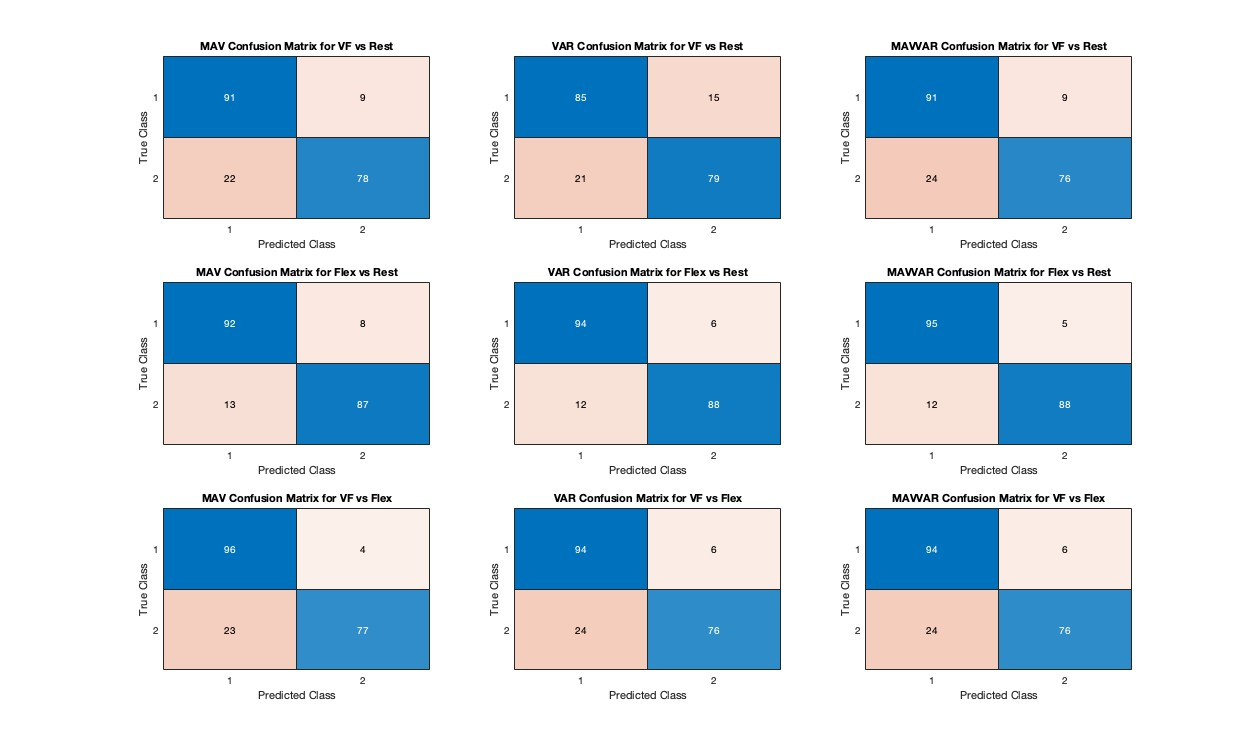
\includegraphics[width=\textwidth]{vf_flex.jpg}
    VF vs. Flex
\end{center}

\begin{center}
    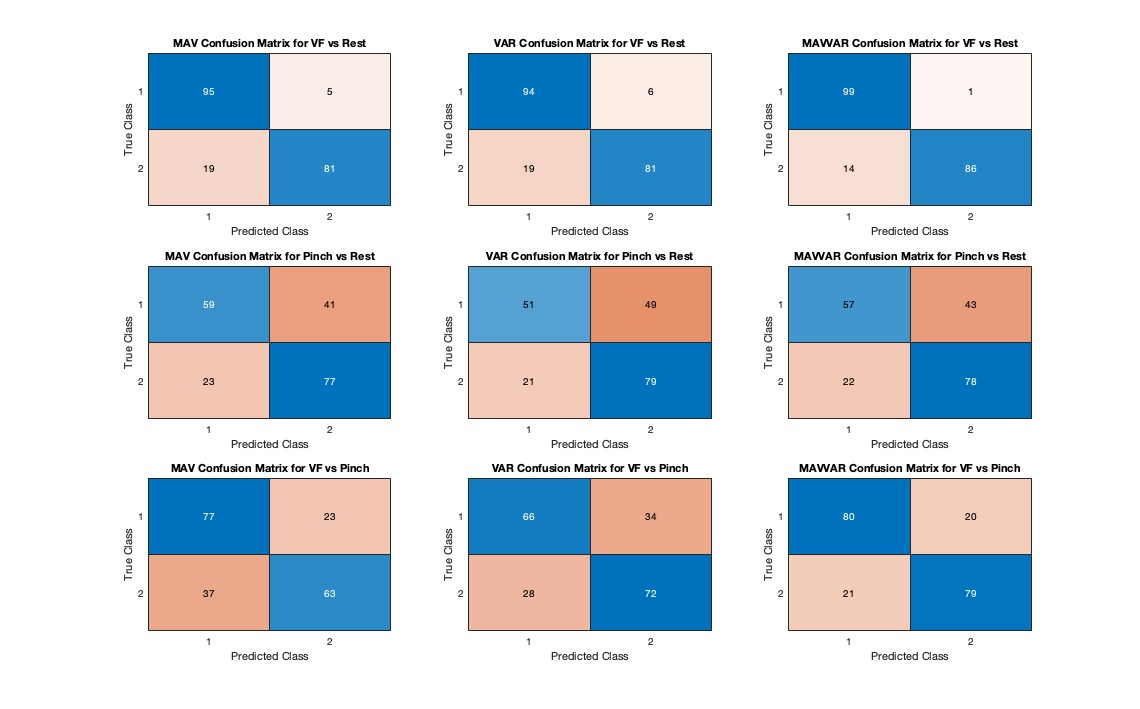
\includegraphics[width=\textwidth]{vf_pinch.jpg}
    VF vs. Pinch
\end{center}

\begin{center}
    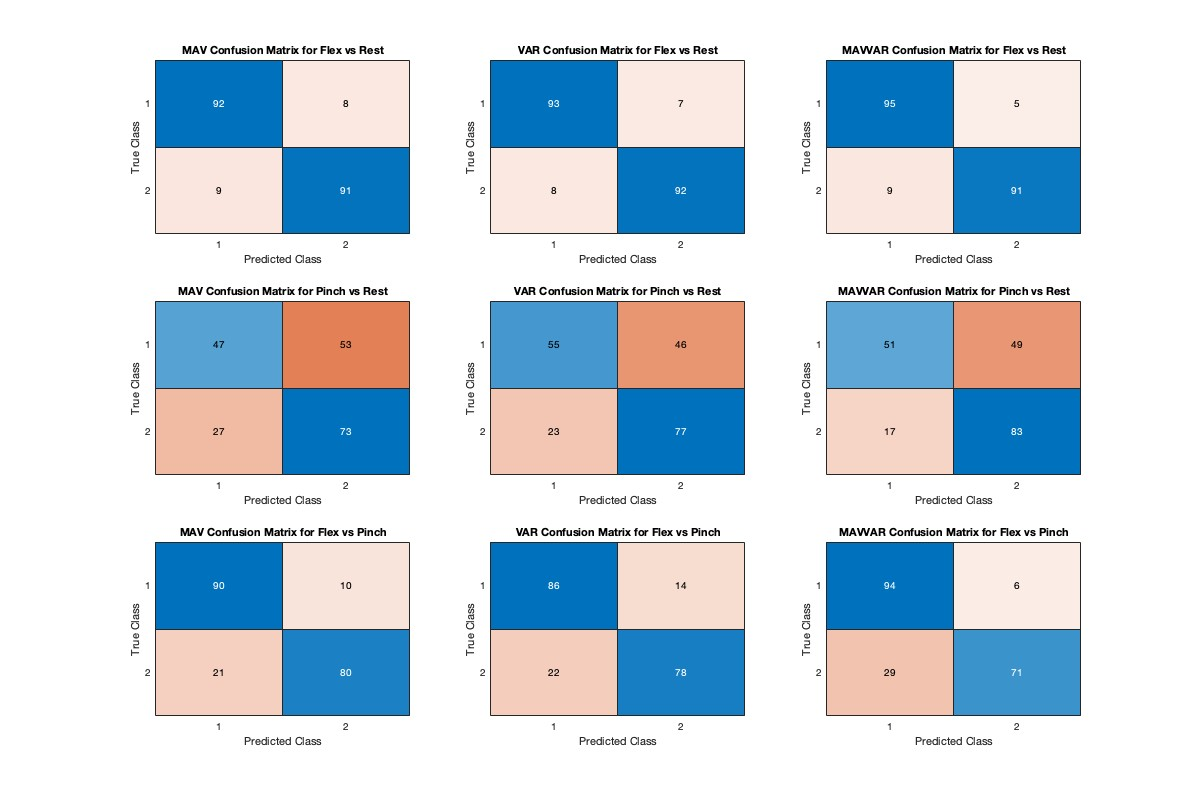
\includegraphics[width=\textwidth]{flex_pinch.jpg}
    Flex vs. Pinch
\end{center}

The confusion matrices show that it was easy to classify VF and Flex against Rest but hard to classify Pinch against Rest. It was also hard to classify VF against Pinch, though classifying VF against Flex and Flex against Pinch were also easy. 

There seemed to be an imbalance in classification difficulty as any classification with Pinch had high confusion, while VF and Flex classifications had low confusion. This tells me that VF and Flex are likely the easiest signals to detect, while Pinch is the hardest. These findings are consistent with the PSD plots since Pinch had a very similar signal to Rest and VF and Flex had a very different signal from its Rest signal. Additionally, this matches the SNR values we found earlier since Pinch had the lowest SNR of all the classes.

Across the board, MAV seemed to have a lower confusion rate than VAR. This is inconsistent with the SNR values we found earlier since VAR had a higher SNR than MAV for all three classes.

Finally, the split of the training and testing sets is not random due to the temporal nature of the data. Randomly shuffling the data would destroy crucial information about the data and produce a classifier that would not generalize well to new data. Splitting the data temporally is a much better approach to allow the classifier to work for new, real-time data.

\end{document}